\noindent \textit{\textcolor{red!60!black}{
Additional comment\\
}}

\textit{\textcolor{red!60!black}{
``They should do a panel, show no pre trends, show that there is no endogenous adjustement in di \textit{(and if none, am at a loss as to why good managers in unconstrained firms did not adjust after September 1931.)}''
}}

\noindent Thank you for raising this interesting point. We found ourselves grappling with the same puzzle as we conducted the empirical analysis for this revision. As documented in our response to Comment 3, the return evidence suggests that the market initially perceived Britain's departure as unfavorable to firms with gold-denominated debt. Yet managers did not respond by redeeming their gold bonds in greater numbers prior to the abrogation.

Providing a definitive answer to this puzzle is challenging. However, by studying US politics and monetary policy during this period, we can offer some perspective. The swift policy response of the Fed following Britain's departure and the policy stances of Presidents Hoover and Roosevelt up to April 1933 can shed some light on the issue. We discuss the chronology of the events below.

According to \cite{Friedman1963}, between September 16 and October 28, speculators (central banks and private holders) converted a substantial amount of their dollar assets to gold anticipating that the US would follow the same path as Great Britain. The joint effect of their action can be seen in Figure \ref{fig:R6_gold_stock}. 

\begin{figure}[h]
  \centering
  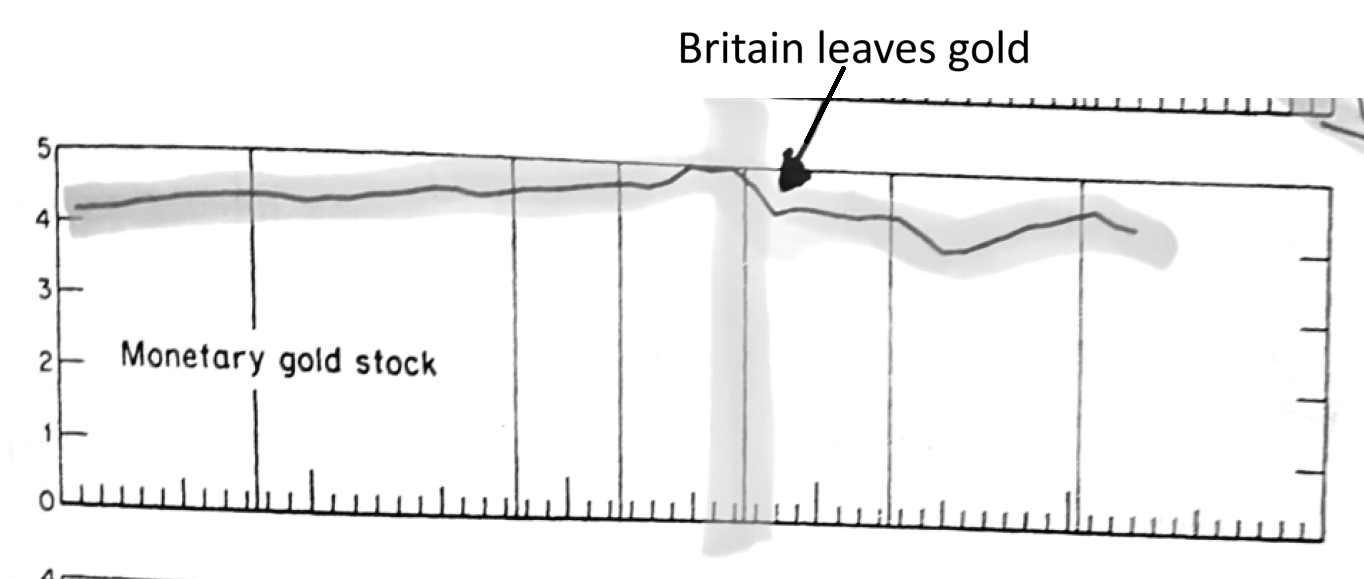
\includegraphics[width=0.8\textwidth]{../../referee-responses-figures/r6-gold-stock.png}
  \caption{US gold stock}
  \label{fig:R6_gold_stock}
\end{figure}

The Federal Reserve System reacted promptly to the drain. On October 9, the bank raised the discount rate to 2.5\% and on October 16, to 3.5\%. Figure \ref{fig:R6_discount_rate} shows the sharp increase in the discount rate in the aftermath of Britain's departure. Following the Fed's move, the gold outflow was contained and the gold stock reached its trough at the end of October.

\begin{figure}[h]
  \centering
  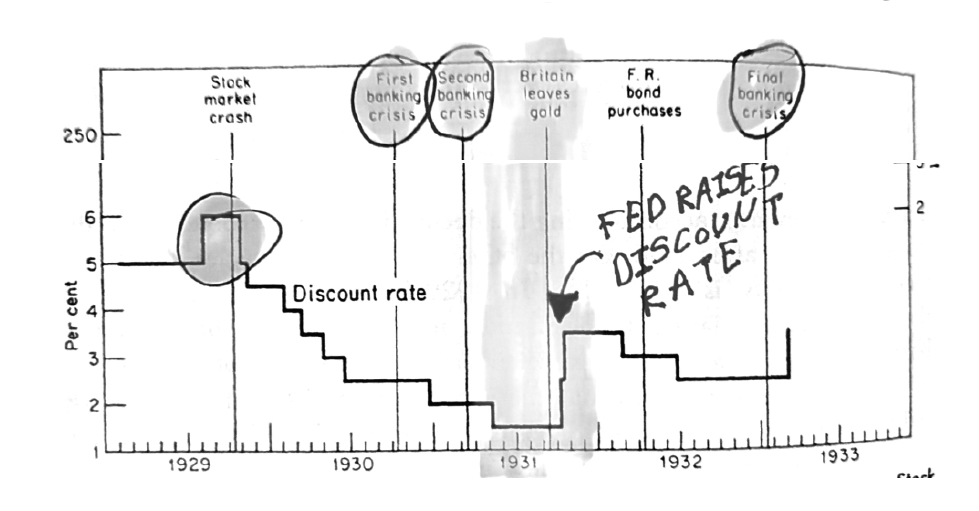
\includegraphics[width=0.8\textwidth]{../../referee-responses-figures/r6-discount-rate.png}
  \caption{FED discount rate}
  \label{fig:R6_discount_rate}
\end{figure}

According to \cite{Friedman1963}, the vigor and promptness of the Fed's actions was unprecedented in its history. The rise in the discount rate was the sharpest and steepest in the history of the Fed, and it arguably discouraged speculators from running on US gold. It is thus conceivable that the decisiveness of the Fed's actions was also enough to persuade managers that the monetary authority was seriously committed to the standard.

These events unfolded within a political context where President Hoover remained a steadfast advocate of the gold standard, which he famously described as "little short of a sacred formula" (\cite{Eichengreen2000}). In multiple speeches, he asserted that the United States possessed both the ability and the moral obligation to maintain the gold standard.

During the 1932 presidential campaign, future president Roosevelt himself emphatically denied that he would alter the value of gold in response to Hoover's claim to the contrary. As late as March 6, 1933, the secretary of the Treasury, Will Woodin, had even reiterated the administration's commitment to the gold standard saying that it was ``ridiculous and misleading to say that we are off the gold standard.... We are definitely on the gold standard.'' Thus, it seems conceivable that the strong bipartisan support the gold standard received up to April 1933 was sufficient to convince firm managers that going off gold wasn't a serious possibility.

Finally, there is also the more mundane aspect of the cost involved in redeeming a firm's outstanding corporate bonds. In those years, bond prices were severely depressed. Figure \ref{fig:R6_bond_quotes} reports quotes (\% of par value) for several industrial corporate bonds at the end of September 1931.

\begin{figure}[h]
  \centering
  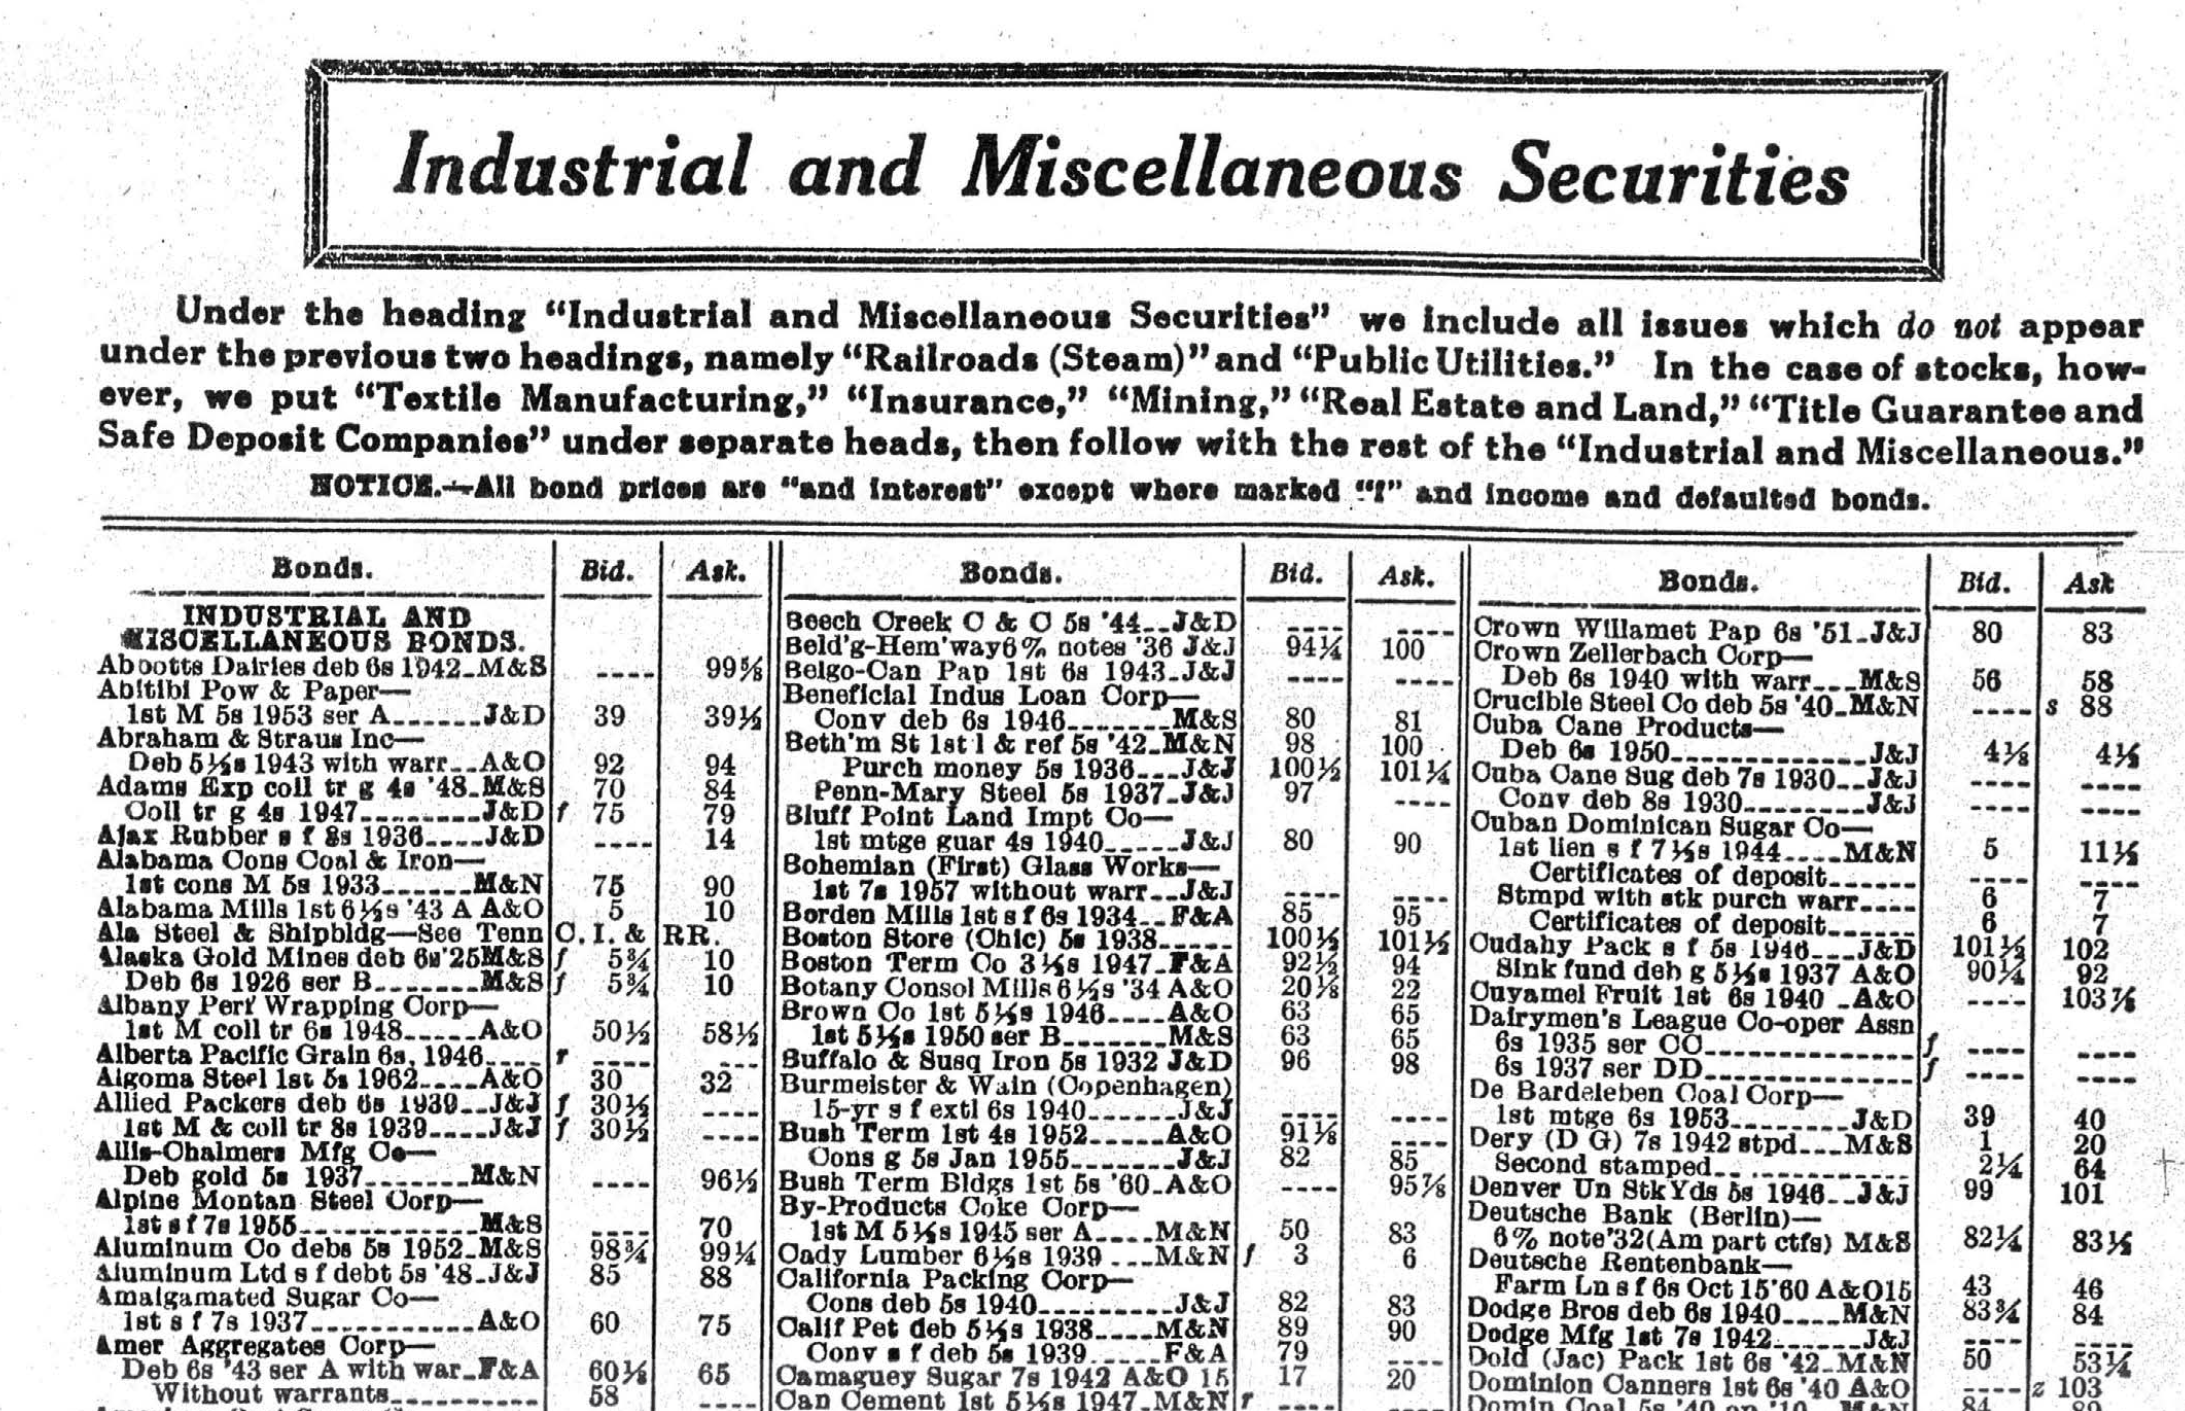
\includegraphics[width=0.9\textwidth]{../../referee-responses-figures/r6-bond-quotes.png}
  \caption{Industrial bond quotes. Commercial and Financial Chronicle, Oct 1931}
  \label{fig:R6_bond_quotes}
\end{figure}

As the figure shows, many of the bonds were traded at a steep discount with respect to their par value of 100. Redeeming the bonds by exercising call options, to the extent that the bond had one, would have been quite costly. The strike price of those options is typically at a premium above par. Purchasing the bonds through open market operations might also have been a costly option given the price impact that a large purchase would likely involve.

For these reasons, while early redemption might have been optimal in the absence of frictions and with perfect foresight, it is plausible that most managers either did not anticipate the abrogation or deemed early redemption too costly.

Thank you again for your constructive and insightful comments. The new analyses, guided by your suggestions, have significantly strengthened the empirical evidence and improved our understanding of the mechanism, providing a more comprehensive perspective on this period. In particular, your questions prompted us to engage more deeply with the political and economic context of the time, from which we have learned a great deal.
